\documentclass{beamer}
\usepackage{beamerthemeCambridgeUS}
\usepackage{color}  % for \textcolor{red}{blah}
\usepackage{graphicx}
\usepackage{subfigure}
\usepackage{multicol}
\usepackage{verbatim} % for \begin{comment}
\usepackage{lipsum}


\newcommand\Fontvi{\fontsize{6}{7.2}\selectfont}


\newenvironment{packed_enum}{
\begin{enumerate}
  \setlength{\itemsep}{1pt}
  \setlength{\parskip}{0pt}
  \setlength{\parsep}{0pt}
}{\end{enumerate}}

\newenvironment{packed_item}{
\begin{itemize}
  \setlength{\itemsep}{1pt}
  \setlength{\parskip}{0pt}
  \setlength{\parsep}{0pt}
}{\end{itemize}}

\usetheme{CambridgeUS}

\title{Discrete Mathematics}
\author[Geoffrey Buhl]{Geoffrey Buhl \\ \texttt{geoffrey.buhl@csuci.edu}}
\institute[CSUCI]{California State University Channel Islands}
\date{week 7 class 1}

\def \vec{{\rm vec}}
\newtheorem{conjecture}[theorem]{Conjecture}
\newtheorem{explanation}[theorem]{Explanation}


\begin{document}

%\frame{\titlepage}

%\section[Outline]{}
%\frame{\tableofcontents}

\frame
{
  \frametitle{Solving Recurrence Relations}

Today we continue  develop a second method for solving recurrence relations, the generating function method.

\vfill
Class Session Goals:
\begin{packed_enum}
\item Practice constructing non-homogeneous recurrence relations.
\item Present Generating Function method for solving non-homogeneous recurrence relations.
\item Demonstrate the Auxiliary equation for repeated roots.
\end{packed_enum}
\vfill
}

\frame
{
  \frametitle{Taylor Series}

The Taylor Series of a function $f(x)$ at $x=0$ is:\\

$$f(0)+f'(0)x+\frac{f''(0)x^2}{2}+\frac{f^{(3)}(0)x^3}{3!}+\frac{f^{(4)}(0)x^4}{4!}+ \cdots=\sum^{\infty}_{n=0}\frac{f^{(n)}(0)x^n}{n!}$$

where $f^{(n)}$ is the $n$th derivative of $f$ evaluated at zero.  If $f(x)$ is {\bf analytic} then $f(x)$ is equal to its Taylor series. That is, if $f$ is analytic

$$f(x)=\sum^{\infty}_{n=0}\frac{f^{(n)}(0)x^n}{n!}$$
}

\frame
{
  \frametitle{Couple more Important Taylor Series}


$$\frac{1}{(1-\alpha x)^2}=1+2\alpha x+3\alpha^2x^2+4\alpha^3x^3+5\alpha^4x^4+6\alpha^5x^5+ \cdots=\sum_{n=0}^{\infty}(n+1)\alpha^nx^n$$
which is obtained by substituting $ \alpha x$ in for $x$ in the Taylor series for $\frac{1}{(1- x)^2}$.\vfill

$$\frac{1}{(1-x)^3}=1+3x+6x^2+10x^3+15x^4+21x^5+ \cdots=\sum_{n=0}^{\infty}\frac{(n+1)(n+2)}{2}x^n$$
which is obtained by differentiating the  Taylor series for $\frac{1}{(1-x)^2}$ and dividing the result by 2.

}

\frame
{
  \frametitle{Generating Function Method Activity}

In small groups, work on the ``Generating Function'' worksheet. The goals of this worksheet are to:
\vfill
\begin{packed_enum}
\item Practice finding a non-homogeneous generating function of a sequence.
\end{packed_enum}
\pause
\vfill
\underline{Problem 1 answer}\\$a_n=2a_{n-1}+2^{n-1}$ with $a_1=1$ (A001787)
%\pause
%\vfill
%\underline{Problem 2 answer}\\ $c_n=a_{n-1}+n$ with $c_0=1$ (A000124)

}

\frame
{
  \frametitle{Binary Matrix sequence}
Let $a_n$ be the number of binary $2 \time 2n$ matrices with exactly $n+1$ 1s and no all zero rows or columns.
$$\left[
   \begin{matrix} % or pmatrix or bmatrix or Bmatrix or ...
      1 & 0 & 1& 0& 1& 0& 1& 0& 1& 1\\
      1 & 1 & 0& 1& 0& 1& 0& 1& 0& 0\\
   \end{matrix}
   \right]
$$ \vfill

Solve $a_n=2a_{n-1}+2^{n-1}$ with $a_1=1$ using the generating function method. \vfill
\pause
Answer $a_n=n 2^{n-1}$ for $n\ge 1$.
}

\begin{comment}
\frame
{
  \frametitle{Lazy Caterer sequence}
  
Let $c_n$ be  the maximum number of pieces you can cut a circular cake into with $n$ vertical cuts. \vfill
  \begin{figure}[htp]
  \begin{center}
    \subfigure{
\includegraphics[scale=.30]{caterer}}
    \end{center}
\end{figure}

Solve $c_n=a_{n-1}+n$ with $c_0=1$ using the generating function method. \vfill
\pause
Answer $c_n=\frac{n(n+1)}{2}+ 1$ for $n\ge 0$.

}
\end{comment}



\frame
{
  \frametitle{Auxiliary Equation with repeated roots}

The recurrence $a_n=2a_{n-1}+2^{n-1}$ with $a_1=1$ is equivalent to the second order homogeneous recurrence $a_n=4a_{n-1}-4a_{n-2}$ with $a_1=1$ and $a_2=4$ (we'll see why next class).  Let's do the auxiliary equation method on this. \vfill
\pause
Again the answer is $a_n=n 2^{n-1}$ for $n\ge 1$.


}

\frame
{
  \frametitle{What if you have more that two equal roots?}

Consider the recurrence relation $b_n=3b_{n-1}-3b_{n-2}+b_{n-3}$ which has auxiliary equation $r^3-3r^2+3r-1=(r-1)^3=0$.  The general solution is $b_n=A1^n+Bn1^n+Cn^21^n$.\vfill

In general, you will have $n^kr^n$ for $k=0, \ldots, n-1$ as terms in the general solution if $r$ appears a root $k$ times in the auxiliary equation.


}

\begin{comment}
\frame
{
  \frametitle{We need a recurrence (or two) }

\vfill
{\bf Problem 1}: Consider tilings $a_n$ of a $1\times n$ board with $1 \times 2$ red tiles, $1 \times 2$ white tiles, $1 \times 2$ blue tiles, $1 \times 1$ orange tiles, and $1 \times 1$ cyan tiles.  What is the recurrence relationship for $a_n$ and what are the initial conditions?
\vfill

{\bf Problem 2}: Consider Problem 1 but with $r$ different colors of $1 \times 2$ tiles and $s$ different colors of $1 \times 1$ blocks.  What is the recurrence relationship to describe the number of tilings $b_n$ of a $ 1 \times n$ board?  What are the initial conditions?
\vfill


}


\frame
{
  \frametitle{We need some recurrence relations}


{\bf  Problem 1}: How many flags with $n$ horizontal stripes can you make with $3$ colors so that adjacent stripes are different colors and the top and bottom stripes are different?
\vspace{.25cm}

{\bf Problem 2}: How many different tiling are there of a $1\times n$ board with $1 \times 1$ white tiles, $2 \times 1$ white tiles, and $2 \times 1$ black tiles?
\vspace{.25cm}

{\bf Problem 3}: How many different tiling are there of a $2\times n$ board with $1 \times 1$  tiles, and right triominos?

}

\frame
{
  \frametitle{We need some more recurrence relations}

%All Jacobsthal sequence

{\bf Problem 1}: How many different tiling are there of a $1\times n$ board with $1 \times 1$ white tiles, $2 \times 1$ white tiles, and $2 \times 1$ black tiles?
\vspace{.25cm}

{\bf Problem 2}: How many different tiling are there of a $2\times n$ board with $2 \times 1$  tiles, and $2 \times 2$  tiles?

{\bf Problem 3}: How many different tiling are there of a $3\times n$ board with $1 \times 1$  tiles, and $2 \times 2$  tiles?
\vspace{.25cm}

{\bf Problem 4}: How many ternary strings of length $n$ are there with no  two consecutive letters are non-zero?
\vspace{.25cm}

}


\frame
{
  \frametitle{Flags}

How many different flags $f_n$ with $n$ horizontal stripes can you make with $3$ colors so that adjacent stripes are different colors?  What is $f_1$, $f_2$ and $f_3$? Find a recurrence relation using the addition principle.  Find a closed form solution with the multiplication principle.

  \begin{figure}[htp]
  \begin{center}
    \subfigure{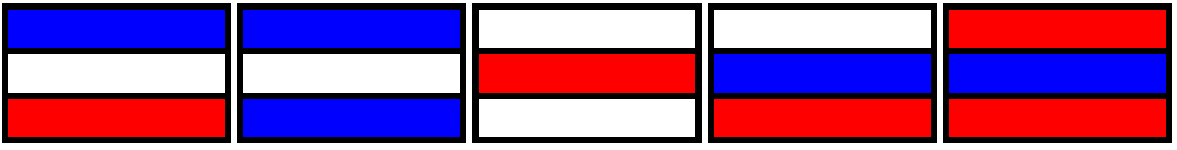
\includegraphics[scale=.45]{flags}}
    \end{center}
\end{figure}

}

\frame
{
  \frametitle{Staircases and Down-Right Paths}



  \begin{figure}[htp]
  \begin{center}
    \subfigure{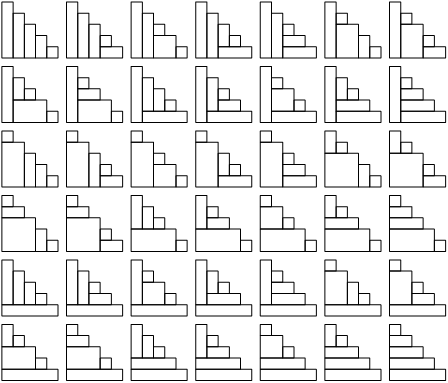
\includegraphics[scale=.38]{Catalan_stairstep_5}}
    \subfigure{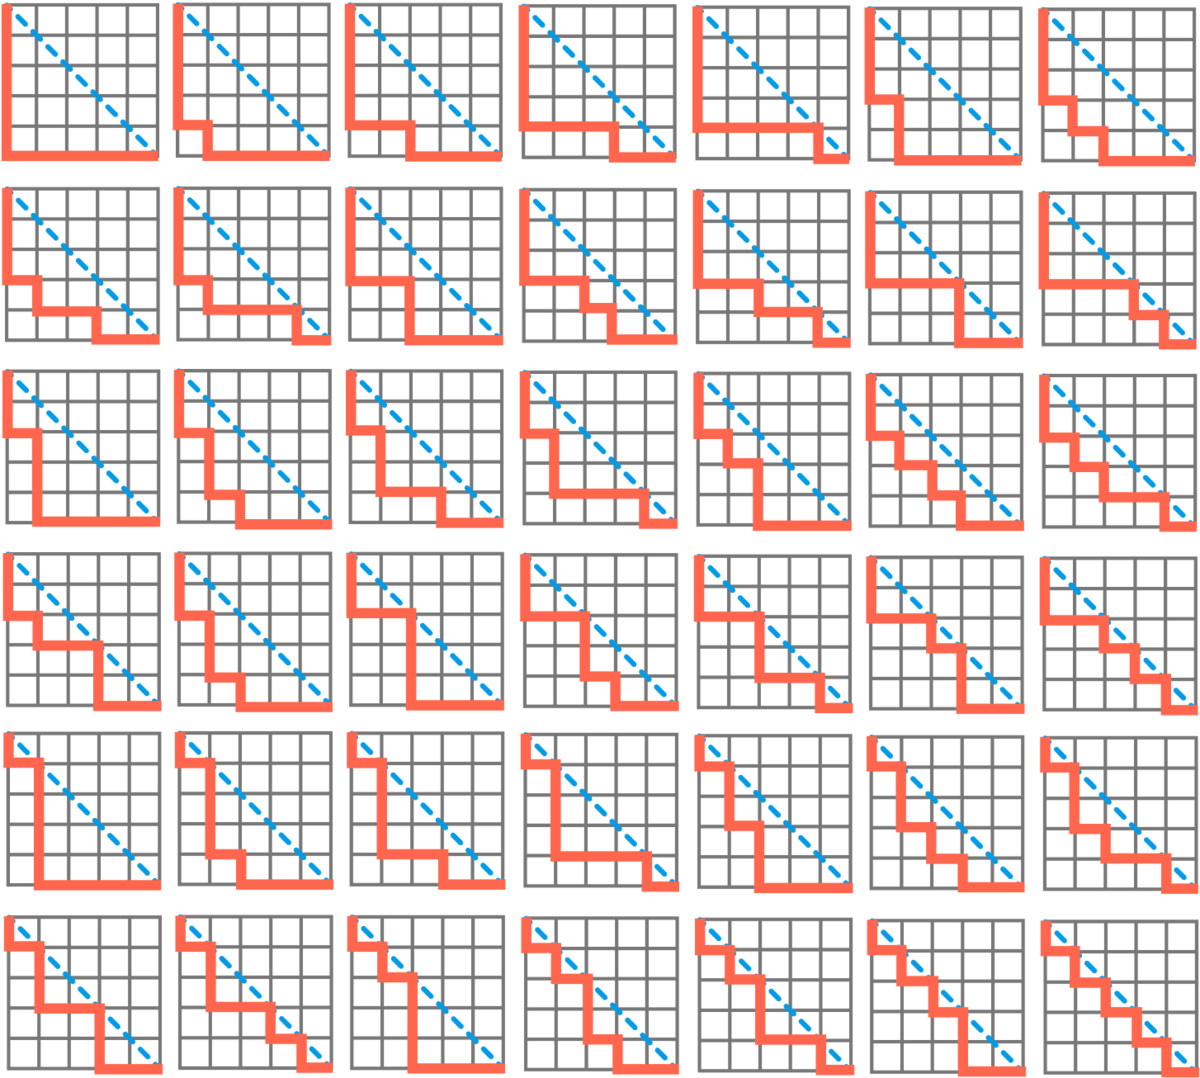
\includegraphics[scale=.135]{dyck_path_5}}
    \end{center}
\end{figure}

}

\frame
{
  \frametitle{$n=6$ Case}
\begin{figure}[htp]
    \subfigure{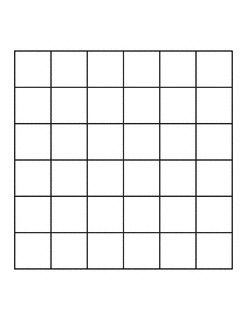
\includegraphics[scale=.75]{66board}}
\end{figure}

}

\end{comment}

\end{document}

